\documentclass[11pt, a4paper, twoside]{article}
\raggedbottom
% questi due pacchetti servono per indicare la codifica della tastiera usata e i caratteri che vogliamo usare.
% a noi non servono molto, ma metti che compiliamo con un computer russo?
\usepackage[T1]{fontenc}
\usepackage[utf8]{inputenc}
%non capisco il perché della metà dei pacchetti kek
\usepackage{blindtext}
\usepackage{geometry}
\usepackage{setspace}
\usepackage{titlesec}
\usepackage{indentfirst}
\usepackage{graphicx}
\usepackage[italian]{babel}
\usepackage{catchfile} % used in \getenv command
\usepackage{multicol}
\usepackage{amsmath}
\usepackage{subcaption}
\usepackage[hang, flushmargin, multiple, bottom]{footmisc}
\usepackage{float}
\usepackage{array}
\usepackage{booktabs}
\usepackage{url}
\usepackage{csvsimple}

\titlespacing*{\section}{0px}{3mm}{1mm}         %what purpouse?
\titlespacing*{\subsection}{0px}{3mm}{1mm}      %what purpouse?
\geometry{
  left=2cm,
  right=2cm,
  top=2cm,
  bottom=2cm
}
\setlength{\parindent}{10mm}
\graphicspath{ {./assets}, {../../assets} }

% Allow use of command \getenv{VARNAME}.
% Taken from: https://tex.stackexchange.com/questions/62010/can-i-access-system-environment-variables-from-latex-for-instance-home
\newcommand{\getenv}[2][]{
  \CatchFileEdef{\temp}{"|kpsewhich --var-value #2"}{\endlinechar=-1}%
  \if\relax\detokenize{#1}\relax\temp\else\let#1\temp\fi}

% Roman numerals
\newcommand{\rom}[1]{\uppercase\expandafter{\romannumeral #1\relax}}

% authors, date and title---------------------------------------------------------------
\author{Giuseppe Sguera \\ \getenv{MAT1} \and Matteo Bonacini \\ \getenv{MAT2}}
\date{\today}
\title{TITOLO}
%---------------------------------------------------------------------------------------
\begin{document}

    %\twocolumn[
    %  \begin{@twocolumnfalse}
        %\begin{center}
{
	{\Large
		{\textsc{Alma Mater Studiorum $\cdot$ Università di Bologna}}
	}
}
\rule[0.1cm]{18cm}{0.1mm}
\rule[0.5cm]{18cm}{0.6mm}
{\small
	{\bf SCUOLA DI SCIENZE\\
		Corso di Laurea in Fisica
	}
}
{\let\newpage\relax\maketitle}
\end{center}


    \maketitle

    \begin{abstract}\label{sec:abstract}
    Lo scopo di questa prova è stato la misurazione della curva caratteristica $I-V$ di un transistor \emph{BJT} in configurazione ad emettitore comune. Abbiamo raccolto tre \emph{set} di dati in corrispondenza di tre diversi valori di corrente di base ($-100, -150, -200 \: mA$). Mediante un \emph{best fit} sono stati calcolati poi conduttanza $g$, guadagno $\beta$ e tensione di Early $V_a$ per ogni curva.
\end{abstract}

    % \end{@twocolumnfalse}
    %]

    \section{Introduzione}\label{sec:textscopo}
Un full adder è un dispositivo che prende come input due bit da sommare più un bit di carry e restituisce in output
un bit di somma e un bit di carry.
L'equazione booleana di questo dispositivo è riportata in appendice \ref{sec:1bfa-equazione}.
Questo dispositivo si può realizzare usando due porte \textsc{exor}, due porte \textsc{and} e una porta \textsc{or}, così come
riportato in figura \ref{fig:circuito}.
È possibile realizzare una porta \textsc{and} e una porta \textsc{exor} in logica positiva usando due diodi e una
resistenza.


    \section{Apparato sperimentale}\label{sec:apparato-sperimentale}
\subsection{Schema del circuito}\label{subsec:schema-circuito}

\begin{figure}[h]
  \centering
      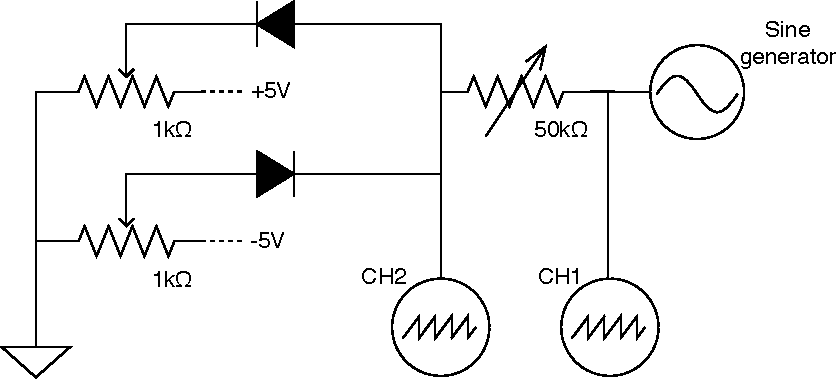
\includegraphics[width=10cm]{../assets/circuito.drawio.pdf}
      \caption{
        \emph{
          Schema del circuito tosatore.
        }
      }
    \label{fig:circuito}
\end{figure}

Il circuito che abbiamo realizzato è schematizzato in figura \ref{fig:circuito}.
È strutturato come segue:
\begin{enumerate}
  \item%
  Due potenziometri da $1k\Omega$ sono collegati a terra e a $\pm 5V$, rispettivamente.
  \item%
  Due diodi al silicio (germanio) sono collegati al pin centrale dei potenziometri.
  \item%
  Un generatore di onda sinusoidale è collegato a una resistenza variabile da $50k\Omega$.
  \item%
  Un canale dell'oscilloscopio vede l'output \emph{pulito} del generatore di funzione.
  \item%
  Un canale dell'oscilloscopio è collegato in parallelo ai due diodi e all'altro capo della resistenza variabile da $50k\Omega$.
\end{enumerate}
Il circuito così realizzato permette di regolare l'ampiezza dell'onda tosata e la curvatura
della porzione tosata.
Per fare ciò, bisogna agire rispettivamente sui due potenziometri da 1k$\Omega$
e sul potenziometro da 50k$\Omega$.

\subsection{Materiale e strumenti usati}\label{subsec:materiali}
Segue una lista del materiale e degli strumenti usati durante la prova:
\begin{itemize}
  \item%
  Oscilloscopio analogico, modello: \emph{GW Instek GOS-652}.
  \item%
  Multimetro digitale, modello: \emph{ISO-TECH IDM 105}.
  \item%
  Generatore di tensione, modello: \emph{Aim-TTi EB2025T}.
  \item%
  Generatore di onda sinusoidale, modello: \emph{GFG-8017G}.
  \item%
  Sonda per oscilloscopio.
  \item%
  Connettori vari (connettori a banana, cavi per la scheda millefori).
  \item%
  2 diodi al silicio
  \item%
  2 diodi al germanio
  \item
  2 potenziometri da $1k\Omega$.
  \item
  Potenziometro da $50k\Omega$.
\end{itemize}

    \section{Risultati}\label{sec:risultati}
Le misure sono state svolte sotto le condizioni riportate in tabella \ref{tab:livelli-logici}.
I risultati dei test delle porte logiche sono riportati di seguente, nelle tabelle \ref{tab:and-fulladder}, \ref{tab:exor-fulladder} e \ref{tab:or-fulladder}.
I risultati delle misure dello 1-bit fulla dder sono riportati in tabella \ref{tab:fulladder}.
I risultati delle misure delle porte \textsc{and} e \textsc{or} sono riportati rispettivamente in tabella \ref{tab:and-logicapositiva} e \ref{tab:or-logicapositiva}.

\begin{table}[H]
  \centering
  \begin{subtable}[H]{0.5\textwidth}
    \centering
    \begin{tabular}[t]{c  c | c  c | c  c}
      \hline
      A & B & V(A) & V(B) & Out & V(Out) (V)\\
      \hline
      0 & 0 & $V_{0}$ & $V_{0}$ & 0 & $0.068 \pm 0.010$ \\
      0 & 1 & $V_{0}$ & $V_{1}$ & 0 & $0.068 \pm 0.010$ \\
      1 & 0 & $V_{1}$ & $V_{0}$ & 0 & $0.068 \pm 0.010$ \\
      1 & 1 & $V_{1}$ & $V_{1}$ & 1 & $4.10 \pm 0.02$ \\
      \hline
    \end{tabular}
  \end{subtable}

  \vspace{.5cm}

  \begin{subtable}[H]{0.5\textwidth}
    \centering
    \begin{tabular}[t]{c  c | c  c | c  c}
      \hline
      A & B & V(A) & V(B) & Out & V(Out) (V)\\
      \hline
      0 & 0 & $V_{0}$ & $V_{0}$ & 0 & $0.070 \pm 0.012$ \\
      0 & 1 & $V_{0}$ & $V_{1}$ & 0 & $0.071 \pm 0.010$ \\
      1 & 0 & $V_{1}$ & $V_{0}$ & 0 & $0.068 \pm 0.010$ \\
      1 & 1 & $V_{1}$ & $V_{1}$ & 1 & $4.09 \pm 0.02$ \\
      \hline
    \end{tabular}
  \end{subtable}

  \vspace{.5mm}

  \begin{subtable}[H]{0.5\textwidth}
    \centering
    \begin{tabular}[t]{c  c | c  c | c  c}
      \hline
      A & B & V(A) & V(B) & Out & V(Out) (V)\\
      \hline
      0 & 0 & $V_{0}$ & $V_{0}$ & 0 & $0.068 \pm 0.010$ \\
      0 & 1 & $V_{0}$ & $V_{1}$ & 0 & $0.068 \pm 0.010$ \\
      1 & 0 & $V_{1}$ & $V_{0}$ & 0 & $0.068 \pm 0.010$ \\
      1 & 1 & $V_{1}$ & $V_{1}$ & 1 & $4.10 \pm 0.02$ \\
      \hline
    \end{tabular}
  \end{subtable}

  \vspace{.5cm}

  \begin{subtable}[H]{0.5\textwidth}
    \centering
    \begin{tabular}[t]{c  c | c  c | c  c}
      \hline
      A & B & V(A) & V(B) & Out & V(Out) (V)\\
      \hline
      0 & 0 & $V_{0}$ & $V_{0}$ & 0 & $0.068 \pm 0.010$ \\
      0 & 1 & $V_{0}$ & $V_{1}$ & 0 & $0.068 \pm 0.010$ \\
      1 & 0 & $V_{1}$ & $V_{0}$ & 0 & $0.068 \pm 0.010$ \\
      1 & 1 & $V_{1}$ & $V_{1}$ & 1 & $4.10 \pm 0.02$ \\
      \hline
    \end{tabular}
  \end{subtable}
  \caption{\emph{Tavole di verità delle porte \textsc{and} corrispondenti ai pin 1-2-3, 4-5-6, 13-12-11, 10-9-8 dell'integrato 7408. I valori di $V_{0}$ e $V_{1}$ sono quelli riportati in tabella \ref{tab:livelli-logici}} sotto la dicitura "F.A.".}
  \label{tab:and1-multiplexer}
\end{table}

\begin{table}[H]
  \centering
  \begin{subtable}[H]{0.5\textwidth}
    \centering
    \begin{tabular}[t]{c  c | c  c | c  c}
      \hline
      A & B & V(A) & V(B) & Out & V(Out) (V)\\
      \hline
      0 & 0 & $V_{0}$ & $V_{0}$ & 0 & $0.068 \pm 0.010$ \\
      0 & 1 & $V_{0}$ & $V_{1}$ & 0 & $0.068 \pm 0.010$ \\
      1 & 0 & $V_{1}$ & $V_{0}$ & 0 & $0.068 \pm 0.010$ \\
      1 & 1 & $V_{1}$ & $V_{1}$ & 1 & $4.10 \pm 0.02$ \\
      \hline
    \end{tabular}
  \end{subtable}

  \vspace{.5cm}

  \begin{subtable}[H]{0.5\textwidth}
    \centering
    \begin{tabular}[t]{c  c | c  c | c  c}
      \hline
      A & B & V(A) & V(B) & Out & V(Out) (V)\\
      \hline
      0 & 0 & $V_{0}$ & $V_{0}$ & 0 & $0.070 \pm 0.012$ \\
      0 & 1 & $V_{0}$ & $V_{1}$ & 0 & $0.071 \pm 0.010$ \\
      1 & 0 & $V_{1}$ & $V_{0}$ & 0 & $0.068 \pm 0.010$ \\
      1 & 1 & $V_{1}$ & $V_{1}$ & 1 & $4.09 \pm 0.02$ \\
      \hline
    \end{tabular}
  \end{subtable}

  \vspace{.5mm}

  \begin{subtable}[H]{0.5\textwidth}
    \centering
    \begin{tabular}[t]{c  c | c  c | c  c}
      \hline
      A & B & V(A) & V(B) & Out & V(Out) (V)\\
      \hline
      0 & 0 & $V_{0}$ & $V_{0}$ & 0 & $0.068 \pm 0.010$ \\
      0 & 1 & $V_{0}$ & $V_{1}$ & 0 & $0.068 \pm 0.010$ \\
      1 & 0 & $V_{1}$ & $V_{0}$ & 0 & $0.068 \pm 0.010$ \\
      1 & 1 & $V_{1}$ & $V_{1}$ & 1 & $4.10 \pm 0.02$ \\
      \hline
    \end{tabular}
  \end{subtable}

  \vspace{.5cm}
  
  \begin{subtable}[H]{0.5\textwidth}
    \centering
    \begin{tabular}[t]{c  c | c  c | c  c}
      \hline
      A & B & V(A) & V(B) & Out & V(Out) (V)\\
      \hline
      0 & 0 & $V_{0}$ & $V_{0}$ & 0 & $0.068 \pm 0.010$ \\
      0 & 1 & $V_{0}$ & $V_{1}$ & 0 & $0.068 \pm 0.010$ \\
      1 & 0 & $V_{1}$ & $V_{0}$ & 0 & $0.068 \pm 0.010$ \\
      1 & 1 & $V_{1}$ & $V_{1}$ & 1 & $4.10 \pm 0.02$ \\
      \hline
    \end{tabular}
  \end{subtable}
  \caption{\emph{Tavole di verità delle porte \textsc{and} corrispondenti ai pin 1-2-3, 4-5-6, 13-12-11, 10-9-8 dell'integrato 7408. I valori di $V_{0}$ e $V_{1}$ sono quelli riportati in tabella \ref{tab:livelli-logici}} sotto la dicitura "F.A.".}
  \label{tab:and2-multiplexer}
\end{table}

\begin{table}[H]
  \centering
  \begin{tabular}[t]{c  c | c  c | c  c}
    \hline
    A & B & V(A) & V(B) & Out & V(Out) (V)\\
    \hline
    0 & 0 & $V_{0}$ & $V_{0}$ & 0 & $0.066 \pm 0.012$ \\
    0 & 1 & $V_{0}$ & $V_{1}$ & 1 & $4.07 \pm 0.14$ \\
    1 & 0 & $V_{1}$ & $V_{0}$ & 1 & $4.07 \pm 0.14$ \\
    1 & 1 & $V_{1}$ & $V_{1}$ & 1 & $4.07 \pm 0.14$ \\
    \hline
  \end{tabular}
  \vspace{.5mm}
  \begin{tabular}[t]{c  c | c  c | c  c}
    \hline
    A & B & V(A) & V(B) & Out & V(Out) (V)\\
    \hline
    0 & 0 & $V_{0}$ & $V_{0}$ & 0 & $0.071 \pm 0.002$ \\
    0 & 1 & $V_{0}$ & $V_{1}$ & 1 & $4.07 \pm 0.14$ \\
    1 & 0 & $V_{1}$ & $V_{0}$ & 1 & $4.07 \pm 0.14$ \\
    1 & 1 & $V_{1}$ & $V_{1}$ & 1 & $4.06 \pm 0.12$ \\
    \hline
  \end{tabular}
  \vspace{.5mm}
  \begin{tabular}[t]{c  c | c  c | c  c}
    \hline
    A & B & V(A) & V(B) & Out & V(Out) (V)\\
    \hline
    0 & 0 & $V_{0}$ & $V_{0}$ & 0 & $0.072 \pm 0.002$ \\
    0 & 1 & $V_{0}$ & $V_{1}$ & 1 & $4.06 \pm 0.12$ \\
    1 & 0 & $V_{1}$ & $V_{0}$ & 1 & $4.06 \pm 0.12$ \\
    1 & 1 & $V_{1}$ & $V_{1}$ & 1 & $4.06 \pm 0.12$ \\
    \hline
  \end{tabular}
  \caption{\emph{Tavole di verità delle porte \textsc{or} corrispondenti ai pin 1-2-3, 4-5-6, 13-12-11 dell'integrato 7408. I valori di $V_{0}$ e $V_{1}$ sono quelli riportati in tabella \ref{tab:livelli-logici}}.}
  \label{tab:or-multiplexer}
\end{table}

\begin{table}[H]
  \centering
  \begin{subtable}
    \centering
    \begin{tabular}[t]{c  c | c  c }
      \hline
      A & V(A) & Out & V(Out) (V) \\
      \hline
      0 & $V_{0}$ & 1 & $4.39 \pm 0.18$ \\
      1& $V_{1}$ & 0 & $0.108 \pm 0.016$ \\
      \hline
    \end{tabular}
  \end{subtable}
  \vspace{.5mm}
  \begin{subtable}
    \centering
    \begin{tabular}[t]{c  c | c  c }
      \hline
      A & V(A) & Out & V(Out) (V) \\
      \hline
      0 & $V_{0}$ & 1 & $4.39 \pm 0.18$ \\
      1& $V_{1}$ & 0 & $0.109 \pm 0.018$ \\
      \hline
    \end{tabular}
  \end{subtable}
  \caption{\emph{Tavole di verità delle porte \emph{not} corrisponenti ai pin 1-2-3, 4-5-6 dell'integrato 7408. I valori di $V_{0}$ e $V_{1}$ sono quelli riportati in tabella \ref{tab:livelli-logici}}.}
  \label{tab:not-multiplexer}
\end{table}

\begin{table}[H]
  \centering
  \begin{tabular}{c c | c c | c c }
    \hline
    $I_{1}$ & $I_{0}$ & $S_{1}$ & $S_{0}$ & Out & V(Out) (V) \\
    \hline
    1 & 0 & 0 & 0 & 0 & $0.07763 \pm 0.00013$ \\
    0 & 1 & 0 & 0 & 1 & $3.85 \pm 0.10$ \\
    0 & 1 & 0 & 1 & 0 & $0.079 \pm 0.018$ \\
    1 & 0 & 0 & 1 & 1 & $3.87 \pm 0.14$ \\
    1 & 1 & 1 & 0 & 0 & $0.0793 \pm 0.0019$ \\
    0 & 0 & 1 & 0 & 1 & $3.78 \pm 0.16$ \\
    1 & 1 & 1 & 1 & 0 & $0.0794 \pm 0.0009$ \\
    0 & 0 & 1 & 1 & 1 & $3.76 \pm 0.12$ \\
  \end{tabular}
  \caption{\emph{Tavola di verità del multiplexer.}}
  \label{tab:multiplexer}
\end{table}

    \section{Conclusioni}\label{sec:conclusioni}
Il circuito realizzato si comporta esattamente come atteso.
Il multiplexer rispetta i valori di tensione di output richiesti: $<0.5V$ per un
segnale \emph{low} e $>2.7V$ per un segnale \emph{high}.
Questo comportamento vale sia per un segnale fisso che per un segnale che varia nel tempo.
    \appendix
  \textbf{\huge{Appendice}}
  \section{Tavola di verità di 1-bit full adder}\label{sec:1bfa-tavola}
  tabella
  \section{Tavola di verità di 1-bit full adder}\label{sec:1bfa-circuito}
  figura


\bibliographystyle{unsrt} % We choose the "plain" reference style
\bibliography{../electronicsLabRefs.bib}

\end{document}
